\documentclass[tikz,border=4pt]{standalone}
\usetikzlibrary{positioning, fit, backgrounds, arrows.meta}

\tikzset{
  gate/.style       = {draw, thick, fill=orange!20, minimum width=9mm, minimum height=6mm},
  op/.style         = {draw, thick, circle, fill=teal!15, minimum size=6mm, inner sep=0pt},
  junction/.style   = {circle, fill, minimum size=1.6mm, inner sep=0pt},
  signal/.style     = {inner sep=1pt},
  cell/.style       = {draw=gray!60, fill=gray!6, rounded corners=6pt, inner sep=4mm},
  cell title/.style = {font=\small\bfseries, text=gray!40!black},
  >={Stealth[length=2mm]},
}

\begin{document}
% One LSTM cell. The gates sit in a row; the cell state c runs along the top,
% forgotten (x) and added to (+); the output h leaves on the right.
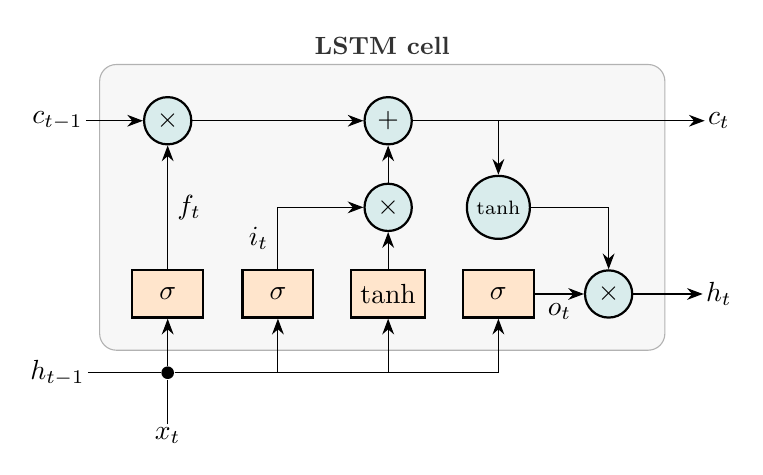
\begin{tikzpicture}[node distance=11mm and 14mm, on grid]
  % The gates: forget, input, candidate, output.
  \node[gate]                         (forget)    {$\sigma$};
  \node[gate]        (inputg) at (1.4,0)    {$\sigma$};
  \node[gate, right=2.8cm of forget]        (candidate) {$\tanh$};
  \node[gate, right=of candidate]     (outputg)   {$\sigma$};

  % Pointwise operations.
  \node[op, above=22mm of forget]     (forgetx)   {$\times$};
  \node[op, above=of candidate]       (inputx)    {$\times$};
  \node[op, above=22mm of candidate]  (plus)      {$+$};
  \node[op, minimum size=8mm, above=of outputg] (squash) {\scriptsize$\tanh$};
  \node[op, right=of outputg]         (outputx)   {$\times$};

  % What comes in and goes out.
  \node[signal, left=of forgetx]      (cprev)     {$c_{t-1}$};
  \node[signal, right=42mm of plus]   (cnext)     {$c_t$};
  \node[junction, below=10mm of forget] (concat)  {};
  \node[signal, left=of concat]       (hprev)     {$h_{t-1}$};
  \node[signal, below=8mm of concat]  (x)         {$x_t$};
  \node[signal, right=of outputx]     (h)         {$h_t$};

  % The cell state.
  \draw[->] (cprev)   -- (forgetx);
  \draw[->] (forgetx) -- (plus);
  \draw[->] (plus)    -- (cnext);
  % h_{t-1} and x_t go to every gate.
  \draw     (hprev)   -- (concat);
  \draw     (x)       -- (concat);
  \draw[->] (concat)  -- (forget);
  \draw[->] (concat)  -| (inputg);
  \draw[->] (concat)  -| (candidate);
  \draw[->] (concat)  -| (outputg);
  % What each gate does.
  \draw[->] (forget)    -- node[right] {$f_t$} (forgetx);
  \draw[->] (inputg)    |- node[pos=0.25, left] {$i_t$} (inputx);
  \draw[->] (candidate) -- (inputx);
  \draw[->] (inputx)    -- (plus);
  \draw[->] (plus)      -| (squash);
  \draw[->] (squash)    -| (outputx);
  \draw[->] (outputg)   -- node[below] {$o_t$} (outputx);
  \draw[->] (outputx)   -- (h);

  \begin{scope}[on background layer]
    \node[cell, fit=(forget) (forgetx) (plus) (squash) (outputx), label={[cell title]north:LSTM cell}] (lstm) {};
  \end{scope}
\end{tikzpicture}
\end{document}
